\usetikzlibrary{positioning}
\definecolor{red}{HTML}{8A3F3A}
\definecolor{yellow}{HTML}{E0BB3C}
\definecolor{blue}{HTML}{4569E0}
\definecolor{green}{HTML}{17E561}
\definecolor{other}{HTML}{6A939E}

% DTU Colors
\definecolor{dtu-corporate-red}{HTML}{990000}
\definecolor{dtu-white}{HTML}{ffffff}
\definecolor{dtu-black}{HTML}{000000}
\definecolor{dtu-blue}{HTML}{2F3EEA}
\definecolor{dtu-bright-green}{HTML}{1FD082}
\definecolor{dtu-navy-blue}{HTML}{030F4F}
\definecolor{dtu-yellow}{HTML}{F6D04D}
\definecolor{dtu-orange}{HTML}{FC7634}
\definecolor{dtu-pink}{HTML}{F7BBB1}
\definecolor{dtu-grey}{HTML}{DADADA}
\definecolor{dtu-red}{HTML}{E83F48}
\definecolor{dtu-green}{HTML}{008835}
\definecolor{dtu-purple}{HTML}{79238E}


\newlength{\basisa}
\setlength{\basisa}{1cm}
\centering
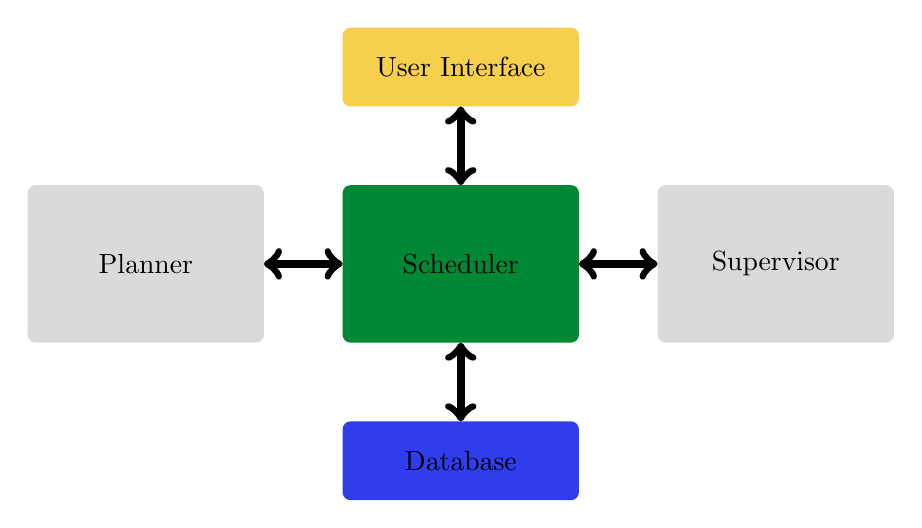
\begin{tikzpicture}[line width=0.0\basisa]
    \draw (4.0\basisa,4.0\basisa) 
		node[minimum height=2\basisa,fill=dtu-grey,minimum width=3\basisa,rounded corners=0.1\basisa] 
			(Planner) {Planner};
    \draw (12.0\basisa,4.0\basisa) 
		node[minimum height=2\basisa,fill=dtu-grey,minimum width=3\basisa,rounded corners=0.1\basisa] 
			(Supervisor) {Supervisor};

			
    \draw (8.0\basisa,4.0\basisa) 
		node[minimum height=2\basisa,fill=dtu-green,minimum width=3\basisa,rounded corners=0.1\basisa] 
			(Scheduler) {Scheduler};
	
    \draw (8.0\basisa,1.5\basisa) 
		node[minimum height=1\basisa,fill=dtu-blue,minimum width=3\basisa,rounded corners=0.1\basisa] 
			(Database) {Database};

    \draw (8.0\basisa,6.5\basisa) 
		node[minimum height=1\basisa,fill=dtu-yellow,minimum width=3\basisa,rounded corners=0.1\basisa] 
			(UserInterface) {User Interface};

	\draw[<->, thick, line width=0.1\basisa] (Planner) -- (Scheduler);
	\draw[<->, thick, line width=0.1\basisa] (Scheduler) -- (Supervisor);
	\draw[<->, thick, line width=0.1\basisa] (Scheduler) -- (Database);
	\draw[<->, thick, line width=0.1\basisa] (Scheduler) -- (UserInterface);
\end{tikzpicture}
